\pagestyle{scrheadings}
\ihead[]{\rightmark}
\ohead[]{Iván Rodríguez Méndez}
\ofoot[]{\thepage{}}
\chapter{Filtros de Kalman}\label{ch:capitulo3}
Una vez hemos comprendido todos los conceptos relacionados con la estimación iterativa de estados pasaremos a describir una importante parte de los estimadores iterativos, los filtros Gaussianos.
% * <amorellg@ull.edu.es> 2016-06-01T17:51:38.815Z:
%
% > recursiva
%
% iterativa
%
% ^ <alu0100765755@ull.edu.es> 2016-06-02T10:49:06.836Z.
Este tipo de filtro en esencia no son más que una aplicación en sistemas continuos de los filtros Bayesianos que vimos en el capítulo 2.
% * <amorellg@ull.edu.es> 2016-06-01T17:52:25.143Z:
%
% > en espacios continuos
%
% parece traducción literal esto, mejor pondría "sistemas contínuos"
%
% ^ <alu0100765755@ull.edu.es> 2016-06-02T10:50:31.298Z:
%
% Efectivamente lo era ! xD
%
% ^ <alu0100765755@ull.edu.es> 2016-06-02T10:50:35.864Z.
Las técnicas utilizadas en los filtros Gaussianos comparten la idea básica de que la certidumbre es representada por distribuciones normales o Gaussianas multivariables.
Recordemos que la expresión para una distribución Gaussiana es la siguiente \cite{thrun_probabilistic_2005}:
\begin{equation}\label{dist_Gauss}
p(x) = det(2\pi \Sigma)^{-\frac{1}{2}}exp(-\frac{1}{2}(x-\mu)^{T}\Sigma^{-1}(x-\mu)) 
\end{equation}
Esta densidad de probabilidad de la variable $x$ está caracterizada por dos parámetros: La media $\mu$ y la covarianza $\Sigma$.
La media típicamente será un vector que tendrá la misma dimensión que el vector de estados $x$. 
Por otra parte la covarianza será una matriz cuadrada, simétrica y positiva.
La dimensión de la matriz de covarianzas será la será $NxN$ si $N$ es la dimensión del vector de estados, por lo tanto el número de elementos presentes en la matriz de covarianzas depende del número de elementos en el vector de estados.

El compromiso para representar la probabilidad a posteriori por medio de una Gaussiana tiene varios enfoques.
Uno de los aspectos más importantes es que la representaciones Gaussianas son unimodales, lo que quiere decir que presentan un único máximo.
Una probabilidad a posteriori de este tipo es característica de muchos problemas de seguimiento en robótica, en la que el 
probabilidad se centra en el estado verdadero con un pequeño margen de incertidumbre.
La probabilidad a posteriori representada por una Gaussiana es una aproximación muy pobre para la mayoría de problemas de estimación global donde pueden existir infinidad de hipótesis, y cada una de ellas puede generar su propia probabilidad a posteriori (problema que resuelven los filtros de partículas).

La presentación de una Gaussiana por medio de su media y su covarianza se conoce como \textit{representación de momentos}.
Esto es así a causa de que la media y la covarianza son el primer y el segundo momento respectivamente de una distribución de probabilidad (los restantes momentos son cero en una distribución normal).
Más adelante hablaremos sobre la \textit{representación canónica} y la \textit{representación natural} de momentos.

\section{Filtro clásico de Kalman (KF)}
Esta herramienta es probablemente la más estudiada en relación a la implementación de filtros Bayesianos.
Como ya explicamos en el capítulo \ref{ch:capitulo2}, el filtro de Kalman fue inventado en la década de los 50 por el matemático Rudolph Emil Kalman. 
Inicialmente se postulaba como una técnica para filtrar y predecir el comportamiento de sistemas lineales.
El filtro de Kalman implementa la certidumbre computacional para estados continuos.
Por lo tanto no sería aplicable a espacios de estados discretos o híbridos.

El \ac{KF} representa en un tiempo $t$ la certidumbre por medio de una media $\mu_{t}$ y una covarianza $\Sigma_{t}$.
La probabilidad a posteriori también será una Gaussiana siempre y cuando las siguientes propiedades se cumplan \cite{thrun_probabilistic_2005}:
\begin{enumerate}
	\item La probabilidad del siguiente estado $p(x_{t} \mid u_{t},x_{t-1})$ debe ser una función lineal afectada con ruido Gaussiano. Lo cual se expresa según la siguiente ecuación (que ya vimos en el capítulo \ref{ch:capitulo2}) que tiene la misma forma que la ecuación \ref{modelodeproceso}:
    \begin{equation}\label{KF_prop_1}
\bar{x}_{t} = A\bar{x}_{t-1} + B u_{t} + w_{t-1} 
	\end{equation}
    \textbf{Donde} $x_{t}$ y $x_{t-1}$ son vectores de estado y $u_{t}$ es el vector de control en el tiempo $t$.
    En la notación que estamos utilizando estos dos vectores son verticales, es decir, están formados de la siguiente manera:
    \begin{equation}\label{vector_estados}
      x_{t} = 
      \left(
      \begin{array}{cccc}
      x_{1,t} \\
      x_{2,t} \\
      \vdots \\
      x_{n,t}
      \end{array}
      \right)
     \end{equation}
     %Insertamos el vector de control
     \begin{equation} \label{Vector_control}
      u_{t} = 
      \left(
      \begin{array}{cccc}
      u_{1,t} \\
      u_{2,t} \\
      \vdots \\
      u_{n,t}
      \end{array}
      \right)
     \end{equation}
     Los elementos $A$ y $B$ de la ecuación \ref{KF_prop_1} son matrices,$A$ es cuadrada $NxN$, donde $N$ es la dimensión del vector de estados $x_{t}$.
     Por otra parte $B$ tiene dimensiones $NxM$, donde $M$ corresponde a la dimensión del vector de control.
     Multiplicando el vector de estados y el de control por las matrices $A$ y $B$ respectivamente la transición de estados se daría de forma \textbf{lineal}.
     Por la razón anterior se asume que el \ac{KF} trabaja con sistemas de \textbf{dinámicas lineales}.
     
     Por otra parte tenemos el factor $\omega_{t-1}$ que como ya comentamos en el capítulo anterior, hace referencia al vector de ruidos Gaussianos que pretende modelar la evolución aleatoria de los estados.
     Este vector deberá tener las mismas dimensiones que el vector de estados.
     Se caracterizan también por tener media cero y  una covarianza no nula denominada $R_{t}$.
     Una transición de estados como la de la ecuación \ref{KF_prop_1} se denomina \textit{lineal-Gaussiana} para resaltar el hecho de que sus argumentos son lineales y está afectada por ruido Gaussiano aditivo. 
     En la ecuación \ref{KF_prop_1} se define la transición de estados en base a la probabilidad $p(x_{t} \mid u_{t},X_{t-1})$, además esta ecuación calcula la media del siguiente estado. 
     Para obtener la covarianza $R_{t}$ tenemos que:
     \begin{equation}\label{Ec:Calcula_Rt}
p(x_{t} \mid u_{t},x_{t-1}) = det(2\pi R_{t})^{-\frac{1}{2}}exp(-\frac{1}{2}(x_{t}-A_{t}x_{t-1}-B_{t}u_{t})^{T}R_{t}^{-1}(x_{t}-A_{t}x_{t-1}-B_{t}u_{t})
	\end{equation} 
     
     \item La probabilidad de las medidas $p(z_{t} \mid x_{t} )$ también debe tener argumentos lineales, con ruido Gaussiano aditivo.
     La ecuación de medida tiene la siguiente forma:
    \begin{equation}\label{Ec:medida}
	z_{t} = C_{t}x_{t}+ \delta_{t}
	\end{equation} 
    Como vemos tiene la misma forma que la ecuación \ref{ecuaciondemedidadeproceso}.
    Aquí $C_t$ es una matriz de dimensiones $KxN$, donde $K$ es la dimensión del vector de medidas $z_{t}$.
    Por otro lado el vector $\delta_{t}$ describe el ruido de medida.
    La distribución de probabilidad de $\delta_{t}$ es multivariable Gaussiana con media cero y covarianza $Q_{t}$.
    La probabilidad en la realización de la medida viene dada por: 
     \begin{equation}\label{Ec:prob_medida}
	p(z_{t} \mid x_{t}) = det(2\pi Q_{t})^{-\frac{1}{2}}exp(-\frac{1}{2}(z_{t}-C_{t}x_{t})^{T}Q_{t}^{-1}(z_{t}-C_{t}x_{t}))
	\end{equation}
    \item Por último, la certidumbre inicial $bel(x_{0})$ seguirá una distribución normal.
% * <amorellg@ull.edu.es> 2016-06-01T17:58:45.933Z:
%
% > debe estar distribuida siguiendo una distribución normal
%
% parece recargado, yo diría "seguirá una distribución normal"
%
% ^ <alu0100765755@ull.edu.es> 2016-06-02T10:55:56.446Z.
    La media de la certidumbre la denominaremos $\mu_0$ y la covarianza como $\Sigma_{0}$.
    La probabilidad la expresamos de la siguiente manera:
     \begin{equation}\label{Ec:prob_certidumbre}
	bel(x_{0})= p(x_{0}) = det(2\pi \Sigma_{0})^{-\frac{1}{2}}exp(-\frac{1}{2}(x_{0}-\mu_{0})^{T}\Sigma_{0}^{-1}(x_{0}-\mu_{0}))
	\end{equation}
\end{enumerate}
\subsection{Algoritmo del KF}

\begin{figure}[ht!]
\centering
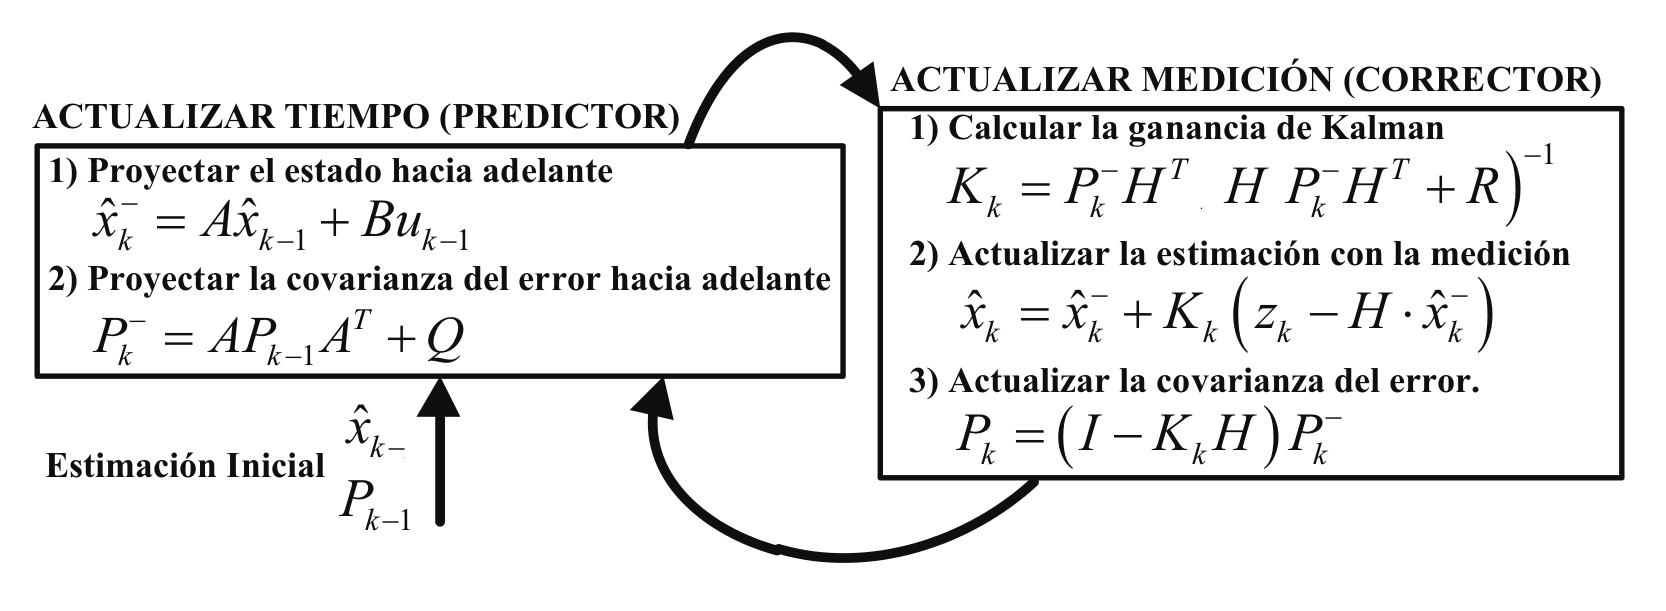
\includegraphics[scale=0.87]{Alg_KF}
\caption{Iteración del KF \cite{leonardo_navegacion_2011}\cite{AnIntroductionToTheKalmanFilter}.} \label{Iteracion_KF}
\end{figure}

Una vez ya tenemos claros todos los principios sobre los que se sostiene el filtro de Kalman clásico, podemos pasar a su implementación en un algoritmo.
\begin{algorithm}
\begin{algorithmic} [1]
\STATE{$\bar{\mu_{t}}=A_{t}\mu_{t-1} + B_{t}u_{t} $}
\STATE{$\bar{\Sigma_{t}}=A_{t}\Sigma_{t-1}A_{t}^{T}+R_{t}$}
\STATE{$K_{t}=\bar{\Sigma_{t}}C_{t}^{T}(C_{t}\bar{\Sigma_{T}}C_{t}^{T}+Q_{t})^{-1}$}
\STATE{$\mu_{t}= \bar{\mu_{t}}+K_{t}(z_{t}-C_{t}\bar{\mu_{t}})$}
\STATE {$\Sigma_{t} = (I-K_{t}C_{t})\bar{\Sigma_{t}}$}
\RETURN $\mu_{t},\Sigma_{t}$
\end{algorithmic}
\caption{Algoritmo KF \cite{thrun_probabilistic_2005} $(\mu_{t-1},\Sigma_{t-1},u_{t},z_{t})$}\label{alg:algoritmoKF}
\end{algorithm}
Podemos ver el planteamiento en el algoritmo \ref{alg:algoritmoKF}.
Las entradas al algoritmo son la certidumbre en un tiempo $t-1$, representada por su media $\mu_{t-1}$ y su covarianza $\Sigma_{t-1}$.
Para la actualización de estos parámetros necesitaremos el vector de control $u_t$ y las medidas tomadas en el instante actual $z_t$.
Podemos ver que la salida del algoritmo es la nueva media $u_t$ y la nueva covarianza $\Sigma_t$ de la certidumbre en el instante $t$. El \ac{KF} es una herramienta muy eficiente a nivel computacional, ya que como podemos apreciar el cálculo matricial que realiza es bastante asequible para cualquier computador.

\begin{figure}[t!]
\centering
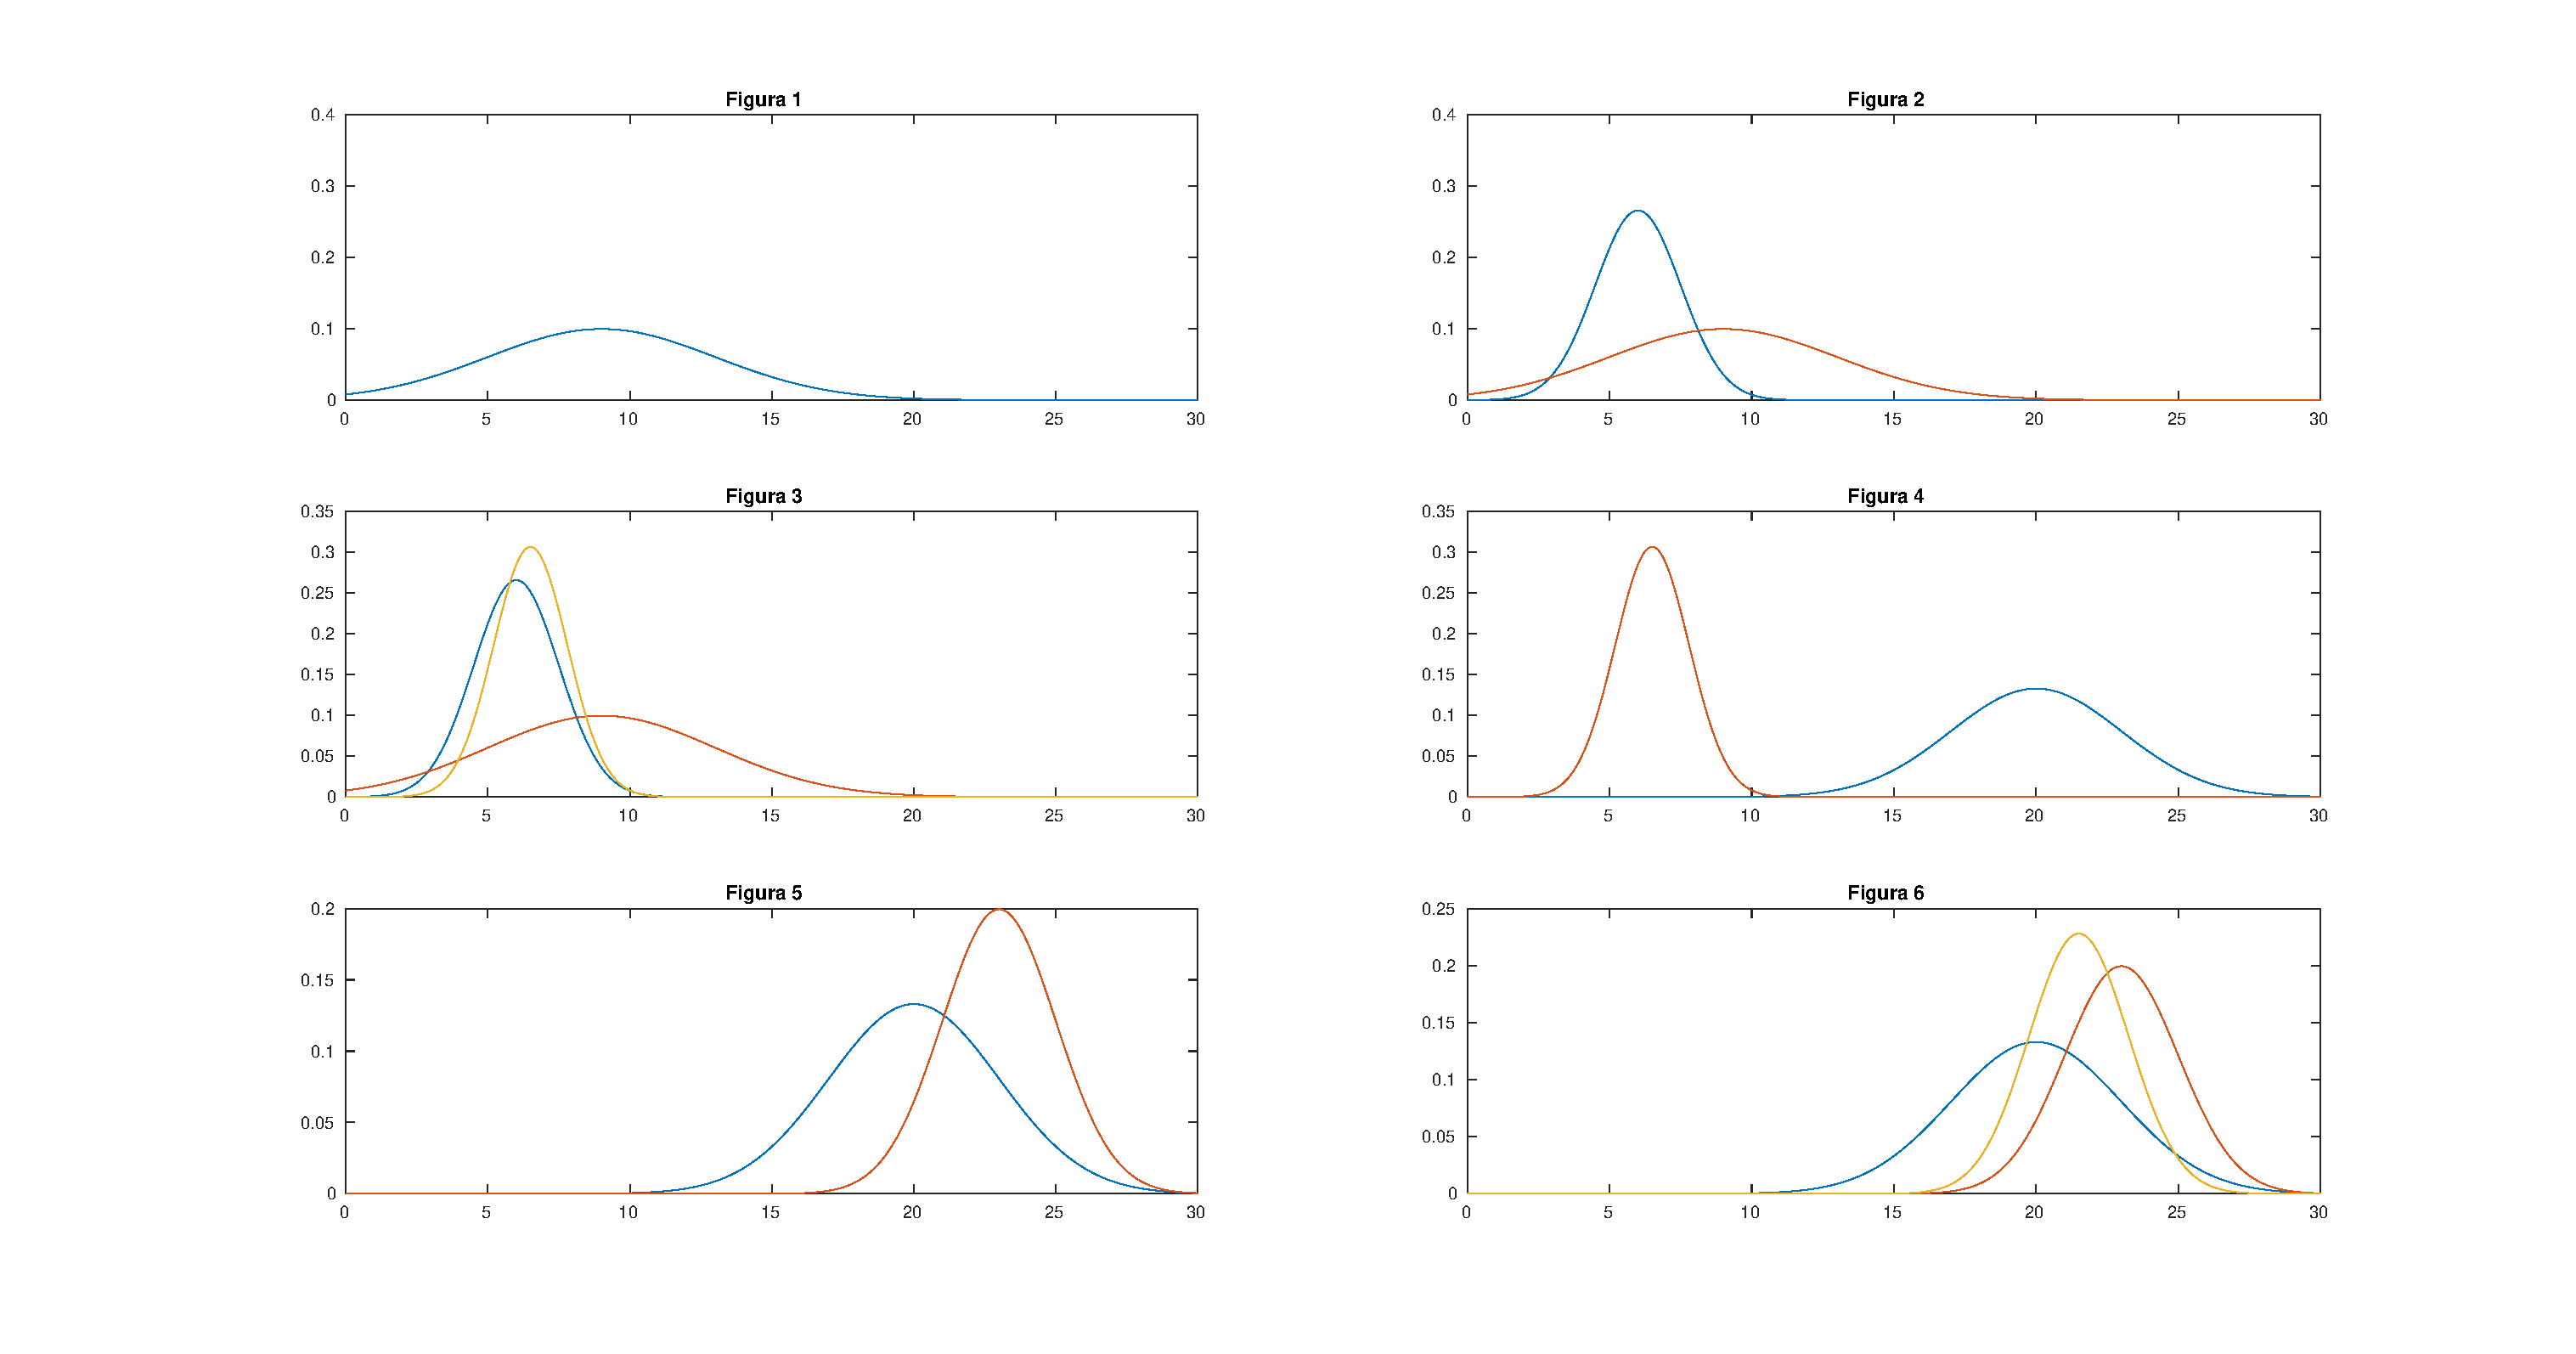
\includegraphics[scale=0.28]{Demostracion-KF}
\caption{Funcionamiento del KF \cite{thrun_probabilistic_2005}.} \label{Demostracion_KF}
\end{figure}

En la figura \ref{Demostracion_KF} muestra un ejemplo simple sobre el funcionamiento del filtro en un espacio unidimensional.
Suponemos que el robot realizará movimientos hacia la derecha en el eje $x$.
La probabilidad a priori de la localización del robot se muestra en la subfigura 1, donde podemos apreciar que la hemos caracterizado siguiendo una distribución Gaussiana.
El robot realizará las medidas del entorno por medio de sus sensores (telémetro, ultrasonidos, etc), y estos devolverán una medida representada mediante otra Gaussiana cuya media será el valor de medida como podemos ver en la subfigura 2.
La Gaussiana de la medida tiene el valor de pico centrado en el devuelto por los sensores, en cuanto a la varianza, esta corresponde a la incertidumbre existente en dicha medida.
Combinando la probabilidad a priori con la medida obtenemos la probabilidad a posteriori que podemos ver en la subfigura 3.
Podemos ver que la certidumbre resultante se encuentra entre las dos medias originales, y la incertidumbre que tiene la nueva Gaussiana es menor que el de las dos Gaussianas anteriores.
El hecho de que las incertidumbre de la Gaussiana resultante sea menor que el de las anteriores puede parecer poco intuitivo.
Este hecho es característico de la integración de la información en el filtro de Kalman donde en general cuanta más información tenemos disponible menos incertidumbre tendremos.

Siguiendo con el ejemplo, ahora suponemos que el robot realiza un movimiento hacia la derecha.
En la subfigura 4 podemos ver como la incertidumbre ha aumentado además de que se ha desplazado en la misma medida que el robot lo ha hecho en el eje hacia la derecha.
En la subfigura 5 el robot vuelve a realizar una medida, que combinada con la probabilidad a priori da como resultado una nueva certidumbre que se muestra en la subfigura 6.
El filtro de Kalman alterna entre el \textit{ciclo de actualización} donde integra las medidas tomadas por lo sensores con el \textit{ciclo de predicción} que modifica la certidumbre conforme a las acciones que ha realizado el robot.
El \textit{ciclo de actualización} reduce la incertidumbre y el \textit{ciclo de predicción} por lo general la aumenta.

\section{Filtro extendido de Kalman (EKF)}
La suposición de que los sistemas tienen transiciones lineales entre estados y que las medidas también son lineales afectadas con ruido Gaussiano aditivo raramente se cumple en la práctica \cite{thrun_probabilistic_2005}.
Un claro ejemplo de la afirmación anterior sería un robot que se mueve con velocidad lineal y angular constante describiendo una trayectoria circular, esta transición de estados no podría ser descrita por ningún tipo de función lineal.
Esta suposición, junto con la suposición de que la certidumbre sigue una distribución unimodal , hace que el KF sea una aproximación demasiado simple, por lo que sería aplicable solamente a problemas triviales de robótica siendo inaplicable en el resto de casos.

El \ac{EKF} supera al \ac{KF} en cuanto a uno de sus supuestos básicos, la linealidad.
En el \ac{EKF} la transición entre estados y las medidas están descritas por funciones no lineales, las funciones $g$ y $h$ respectivamente \cite{thrun_probabilistic_2005}:
\begin{equation}\label{Ec:Estados_EKF}
x_{t}= g(u_{t},x_{t-1})+ \varepsilon_{t}
\end{equation}
\begin{equation}\label{Ec:Medida_EKF}
z_{t}= h(x_{t}) + \delta_{t}
\end{equation}
Este modelo estrictamente generaliza el modelo lineal Gaussiano en el que se basa el \ac{KF}, este modelo lo podemos ver en las ecuaciones \ref{KF_prop_1} y \ref{Ec:medida}.
La función $g$ 
remplaza las matrices $A_{t}$ y $B_{t}$ de la ecuación \ref{KF_prop_1}, y $h$ reemplaza la matriz $C_{t}$ en la ecuación \ref{Ec:medida}.
La evolución de los estados al usar matrices $g$ y $h$ seleccionadas arbitrariamente no presentan una certidumbre distribuida siguiendo una Normal como si ocurría en el \ac{KF}.
De hecho, la realización de la actualización de la certidumbre es normalmente imposible de desarrollar para funciones no lineales $g$ y $h$, ya que los filtros Bayesianos no tienen un método para efectuar este cálculo.
% * <amorellg@ull.edu.es> 2016-06-01T18:10:04.407Z:
%
% > De hecho, la realización de la actualización de la certidumbre es normalmente imposible de realizar para funciones no lineales $g$ y $h$, ya que los filtros Bayesianos no tienen un método para la realización de este cálculo.
%
% "realizar" 3 veces en la misma frase, molaría poner sinónimos
%
% ^ <alu0100765755@ull.edu.es> 2016-06-02T10:57:07.175Z:
%
% Hecho !
%
% ^ <alu0100765755@ull.edu.es> 2016-06-02T11:06:00.540Z.

El \ac{EKF} calcula una aproximación a la certidumbre real por medio de una distribución Gaussiana.
En particular, la certidumbre $bel(x_{t})$ en un tiempo $t$ es representada por una media $\mu_{t}$ y una covarianza $\Sigma_{t}$ como ya explicamos en el capítulo \ref{ch:capitulo2}.
Así el \ac{EKF} hereda del \ac{KF} la forma de representar la certidumbre, pero se diferencia en que esta será una mera aproximación y no es calculada como en el \ac{KF}.

\subsection{Linealización mediante la expansión de Taylor }

Como ya hemos dicho uno de los puntos básicos del \ac{EKF} es la representación de la certidumbre mediante una aproximación de esta.
Por lo tanto la idea principal es la \textit{linealización}.
Si suponemos que tenemos una función no lineal $g$ una función Gaussiana proyectada a través de esta función se convertirá en no Gaussiana.
Esto es porque existen no linealidades en $g$ que perturban la certidumbre de tal manera que hacen que no puede ajustarse a una Gaussiana.
Por lo tanto con la linealización lo que buscamos es aproximar la función $g$ con una función lineal que sea tangente a la función $g$ en la media de la Gaussiana.
Proyectando la Gaussiana por medio de esta aproximación lineal, la distribución de probabilidad a posteriori si será una Gaussiana.
% * <amorellg@ull.edu.es> 2016-06-01T18:11:54.614Z:
%
% > posterior
%
% otras veces te has referido como "a posteriori", usar "posterior" igual puede llevar a confusión
%
% ^ <alu0100765755@ull.edu.es> 2016-06-02T11:06:16.671Z.
De hecho, una vez que $g$ ha sido linealizada el método para la propagación de la certidumbre es igual que para el \ac{KF}.
La misma explicación se aplica a la multiplicación de Gaussianas cuando se utiliza la función $h$.
Para este caso el \ac{EKF} vuelve a aproximar la función $h$ por medio de una función lineal que es tangente a $h$, manteniendo así la naturaleza Gaussiana de la probabilidad a posteriori.

A la hora de linealizar funciones no lineales pueden utilizarse una gran variedad de técnicas.
En concreto el \ac{EKF} utiliza un método llamado \textbf{expansión de Taylor} \cite{_taylor_2016}.
En el \ac{EKF} se suelen trabajar con expansiones de primer y segundo orden.
La expansión de Taylor constituye una aproximación lineal a una función g por medio del valor de sus derivadas y su pendiente.
La pendiente viene dada por la derivada parcial siguiente:
\begin{equation}\label{Ec:Taylor_1}
g'(u_{t},x_{t-1}) := \frac{\partial g(u_{t},x_{t-1})}{\partial x_{t-1}}
\end{equation}
Está claro que el valor de g y su pendiente dependerá de los argumentos de $g$ (vector de estados y de control).
Una elección lógica para seleccionar los argumentos es elegir el estado que se considera más probable en el instante en el que se realiza la linealización.
Para las distribuciones Gaussianas, el estado más probable es la media del posterior estado de control $u_{t-1}$.
En otras palabras, $g$ es aproximada por su valor en el instante en que se da $u_{t-1}$ (y $u_t$).
La linealización por tanto se conseguiría de la siguiente forma:
\begin{equation}\label{Ec:Taylor_2}
g(u_{t},x_{t-1}) \approx g(u_{t},\mu_{t-1}) + g'(u_{t},\mu_{t-1})(x_{t-1}-\mu_{t-1}) 
= g(u_{t},\mu_{t-1}) + G_{t}(x_{t-1}-\mu_{t-1})
\end{equation}
Si lo escribimos utilizando la expresión de una Gaussiana tendríamos:
\begin{eqnarray}\label{Ec:Prob_Taylor}
\nonumber p(x_{t} \mid u_{t},x_{t-1}) \approx \\
\nonumber det(2\pi R_{t})^{-\frac{1}{2}}exp(-\frac{1}{2}[x_{t}-g(u_{t},\mu_{t-1})-G_{t}(x_{t-1}-\mu_{t-1})]^{T} \\
R_{t}^{-1}[x_{t}-g(u_{t},\mu_{t-1})-G_{t}(x_{t-1}-\mu_{t-1})])
\end{eqnarray}
La matriz $G_{t}$ es una matriz de dimensiones $nxn$, donde $n$ es la dimensión del vector de estados.
Esta matriz se conoce con el nombre de \textbf{Jacobiano}.
El valor del Jacobiano depende de $u_{t}$ y $u_{t-1}$, por lo tanto se diferencia para distintos instantes de tiempo.

La misma linealización es implementada para la función de medida $h$.
En esta expresión la serie de Taylor se desarrolla alrededor de $\bar{\mu_{t}}$, que es el estado que se considera más probable para linealizar la función de la siguiente manera:
\begin{eqnarray}\label{Ec:Prob_Taylor_h}
\nonumber h(x_{t}) \approx h(\bar{\mu_{t}}) + h'(\bar{\mu_{t}})(x_{t}-\bar{\mu_{t}}) \\
= h(\bar{\mu_{t}}) + H_{t}(x_{t}- \bar{\mu_{t}}) 
\end{eqnarray}
Sabiendo que $h'(x_{t})=\frac{\partial h(x_{t}}{\partial x_{t}}$ podemos escribir la expresión en forma de Gaussiana:
\begin{eqnarray}\label{Ec:Prob_Taylor_h_Gauss}
\nonumber p(z_{t} \mid x_{t}) = det(2\pi Q_{t})^\frac{-1}{2} exp(-\frac{-1}{2}[z_{t}-h(\bar{\mu_{t}})-H_{t}(x_{t}-\bar{\mu_{t}}]^{T} \\
Q_{T}^{-1}[z_{t}-h(\bar{\mu_{t}})-H_{t}(x_{t}-\bar{\mu_{t}})])
\end{eqnarray}

De esta manera aplicariamos los desarrollos de Taylor en el \ac{EKF} y podríamos seguir usando los supuestos de que las certidumbres vienen dadas por distribuciones Gaussianas.

\subsection{Algortimo del EKF}
\begin{figure}[ht!]
\centering
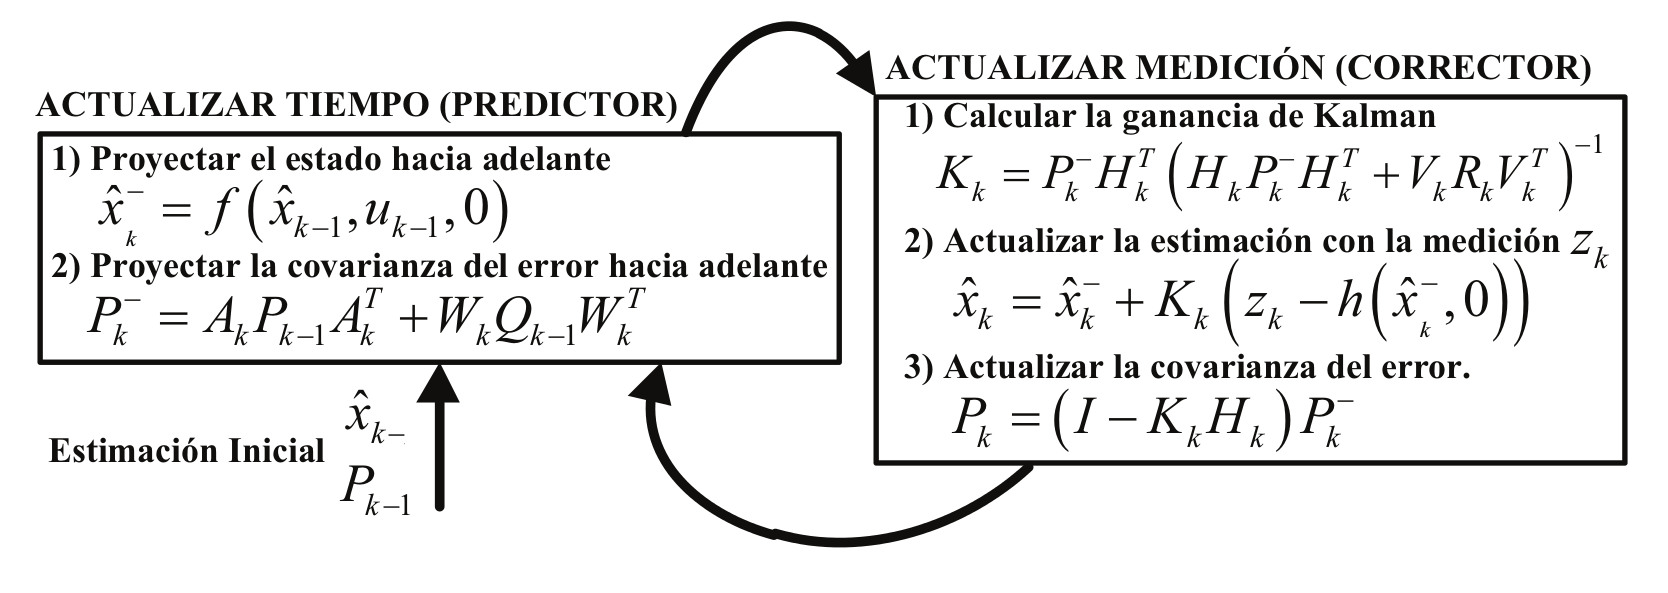
\includegraphics[scale=0.87]{Alg_EKF}
\caption{Iteración del EKF \cite{leonardo_navegacion_2011} \cite{AnIntroductionToTheKalmanFilter}.} \label{Iteracion_EKF}
\end{figure}
\begin{algorithm}
\begin{algorithmic} 
\STATE{$\bar{\mu_{t}}= g(u_{t},\mu_{t-1}) $}
\STATE{$\bar{\Sigma_{t}}=G_{t}\Sigma_{t-1}G_{t}^{T}+R_{t}$}
\STATE{$K_{t}=\bar{\Sigma_{t}}H_{t}^{T}(H_{t}\bar{\Sigma_{t}}H_{t}^{T}+Q_{t})^{-1}$}
\STATE{$\mu_{t}= \bar{\mu_{t}}+K_{t}(z_{t}-h(\bar{\mu_{t}}))$}
\STATE {$\Sigma_{t} = (I-K_{t}H_{t})\bar{\Sigma_{t}}$}
\RETURN $\mu_{t},\Sigma_{t}$
\end{algorithmic}
\caption{Algoritmo EKF \cite{thrun_probabilistic_2005} $(\mu_{t-1},\Sigma_{t-1},u_{t},z_{t})$}\label{alg:algoritmoEKF}
\end{algorithm}

En el algoritmo \ref{alg:algoritmoEKF} y la figura \ref{Iteracion_EKF} podemos ver las ecuaciones que usa el \ac{EKF} para funcionar.
Como podemos apreciar este algoritmo es muy parecido al algortimo \ref{alg:algoritmoKF} donde se aplicaba el \ac{KF}.
Las diferencias más importantes las podemos apreciar en las líneas 1 y 4 en ambos algoritmos.
La predicción del estado (línea 1) en el \ac{KF} se realiza de la forma $A_{t}\mu_{t-1}+ B_{t}\mu_{t}$ mientras que en el \ac{EKF} se realiza de la forma $g(u_{t},\mu_{t-1})$ por lo tanto la predicción de los estados se calculan de forma diferente.
Por otra parte también se diferencian en la predicción de la medida (línea 4) en el \ac{KF} se expresa como $C_{t}\bar{\mu_{t}}$ mientras que en el \ac{EKF} se define como $h(\bar{\mu_{t}})$.

Podemos ver que la predicción lineal usada en el \ac{KF} ha sido reemplazada por expresiones no lineales en el \ac{EKF}.
Además, el filtro extendido de Kalman usa los Jacobianos $G_{t}$ y $H_{t}$ en lugar de las matrices lineales $A_{t}$,$B_{t}$ y $C_{t}$ presentes en el filtro clásico de Kalman.
El Jacobiano $G_{t}$ en el \ac{EKF} corresponde a las matrices $A_{t}$ y $B_{t}$ del \ac{KF}, por otro lado el Hessiano $H_{t}$ corresponde a la matriz $C_{t}$.

\section{ Filtro \textit{unscented} de Kalman (UKF)}
El filtro \ac{UKF} es una formulación para sistemas no lineales \cite{julier_new_2000} al igual que el \ac{EKF} pero sin utilizar la forma de linealizar el sistema de este último.
La diferencia básica está en la manera en la que las variables aleatorias Gaussianas que modelan el ruido son representadas y propagadas a través de la dinámica del sistema.
El \ac{UKF} resuelve este problema por medio de un muestreo determinista.
El \ac{UKF} mantiene la estructura de predicción-corrección tanto del \ac{KF} como del \ac{EKF} que podemos ver en las figuras \ref{Iteracion_KF} y \ref{Iteracion_EKF} pero la forma de realizar el cálculo es diferente.
En lugar de estimar la covarianza del error $\Sigma_{k}^{-}$ utilizando el procedimiento del \ac{EKF}, se hace uso de lo que se conoce como transformación Unscented (UT) \cite{julier_new_2000} que calcula un conjunto de puntos de muestra, conocidos como \textbf{puntos Sigma}, para representar de forma más precisa la media y la varianza del estado ( suponiendo que esta tiene una distribución Gaussiana).
Si propagamos estos puntos a través del sistema no lineal de las ecuaciones \ref{Ec:Estados_EKF} y \ref{Ec:Medida_EKF} la media y la covarianza posterior se obtiene para cualquier no-linealidad presente en el sistema de forma precisa, dando un mejor resultado si lo comparamos con la linealización realizada en el \ac{EKF} tal y como podemos ver en la figura \ref{EKF_UKF_UT}   \cite{julier_general_1996} \cite{julier_new_1995} \cite{julier_unscented_2004}.
Los valores de los puntos sigma (que son escogidos cuidadosamente) se utilizan para obtener la predicción del estado y de su covarianza en una estimación \textit{a priori}.
El \ac{UKF} se postula como un filtro muy preciso en cuanto a la estimación de estados (se trataría de una aproximación de segundo orden), sin embargo, es muy costoso en términos de potencia de cálculo necesaria ya que el algortimo de este filtro necesita calcular la raíz cuadrada de la matriz $\Sigma_{k}^{-}$ aunque por otra parte no es necesario el cálculo del Jacobiano ni del Hessiano.
El \ac{UKF} no podría ser implementado en robots con recursos limitados ya que para estos llevaría mucho tiempo tratar de calcular la operación anterior.

\begin{figure}[ht!]
\centering
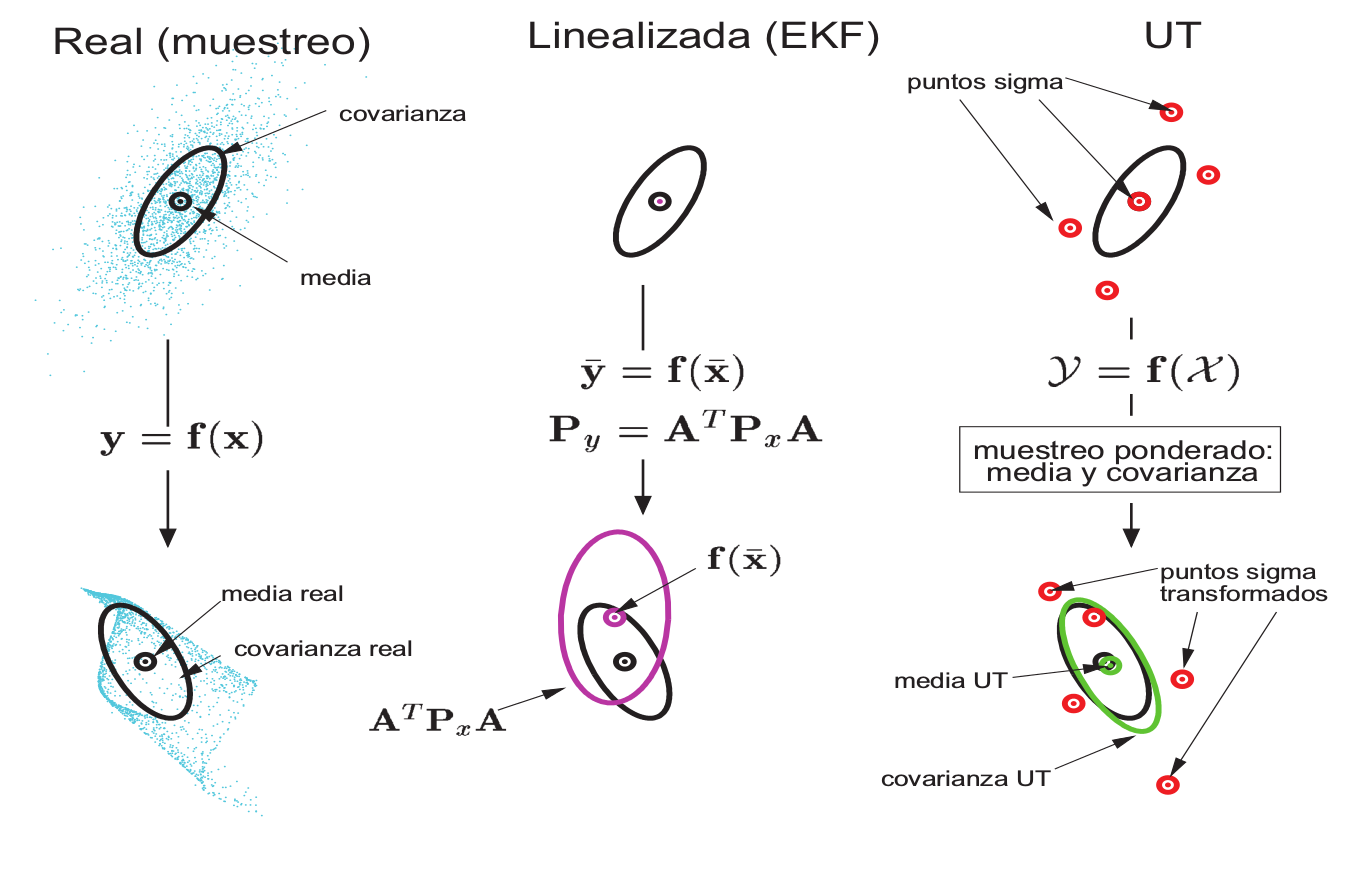
\includegraphics[scale=0.95]{EKF_UT}
\caption{Comparativa linealización y transformada UT \cite{leonardo_navegacion_2011} \cite{wan_unscented_2000} .} \label{EKF_UKF_UT}
\end{figure}

\subsection{La transformación \textit{unscented} (UT)}

La predicción de los estados futuros de un sistema puede calcularse de distintas formas, la transformada UT es uno de ellas.
Suponiendo que $x$ es un variable aleatoria con media $\mu_{x}$ y covarianza $\Sigma_{x}$ una segunda variable aleatoria $y$ se podría relacionar con $x$ por medio de la función no lineal:
\begin{equation}\label{Ec:Trans_UT_1}
y = f(x)
\end{equation}
A la función anterior le podemos calcular a su vez la media ($\mu_{y}$) y la covarianza ($\Sigma_{y}$).
Los distribución de probabilidad de la variable transformada es consistente si se satisface la desigualdad \cite{_leyton_2009} \cite{julier_unscented_2004} en términos de la covarianza y la media de la expresión siguiente:
\begin{equation}\label{Ec:Trans_UT_2}
\Sigma_{y}- E[(y-\mu_{y})(y-\mu_{y})^{T}] \ge 0
\end{equation}
Si no se cumple la condición \ref{Ec:Trans_UT_2} se podrá considerar a $\Sigma_{y}$ subestimada.
Sin embargo, la consistencia no necesariamente implica que vayamos a obtener buenos resultados ya que los cálculos finales están sujetos a la minimización del error cuadrático medio.

La transformada \textit{unscented} es un novedoso método utilizado para calcular la distribución de probabilidad de una variable aleatoria que ha sido sometida a una transformación no lineal.
Este método se basa en la idea de que es más fácil aproximar una distribución Gaussiana que aproximar una función no lineal arbitraria \cite{julier_new_1995}. 
El método consiste en elegir un conjunto de puntos llamados \textbf{puntos sigma}, con la condición de que su media y covarianza coincida con las de la variable aleatoria $x$ del proceso.
A continuación, la transformación no-lineal $f$ se aplica a cada punto sigma y a estos puntos $(y=f(x))$ se les calcula la esperanza $E[y]$ y la covarianza $\Sigma_{y}$.

Si $x$ es una variable aleatoria de dimensión $L$ con media $E[x] = \mu_{x}$ y covarianza $\Sigma_{x}$, entonces para calcular la media $E[y]=\mu_{y}$ y la covarianza $P(y) = \Sigma_{y}$ se construye la matriz de puntos sigma $\chi_{0}$ con $(2L+1)$ vectores columna \cite{houshangi_accurate_2005} \cite{chow_unscented_2007} resultando:

\begin{eqnarray}\label{Ec:Chi_UKF_UT}
\nonumber \chi_{0} = \mu_{x} \\
\nonumber \chi_{i} = \mu_{x} + (\sqrt[]{(L+ \lambda)\Sigma_{x}})_{i} ; i=1,\cdots,L \\
\chi_{i} = \mu_{x} - (\sqrt[]{(L+ \lambda)\Sigma_{x}})_{i-L} ; i=L+1,\cdots,2L 
\end{eqnarray}
donde $\delta = \alpha^{2}(L+k)-L$ y $\alpha$ (generalmente $1x10^{-4} \le \alpha \le 1 $) determinan la dispersión de los puntos alrededor de $\mu_{x}$, $k$ es una constante relacionada con el parámetro de escala (generalmente $0 \le k \le 3-L$) y $(\sqrt[]{(L+ \delta)\Sigma_{x}})$ es la i-ésima columna de la matriz cuadrada $(L+ \delta)\Sigma_{x}$.

El cálculo de la media y la covarianza de la variable aleatoria también se puede lograr mediante la utilización de una descomposición de Cholesky \cite{oh_development_2006} \cite{_leyton_2009} y será en definitiva la que se utilizará para la implementación que se realiza en la toolbox \cite{toolbox_simo} del \ac{UKF}.

Se puede comprobar que los puntos sigma contienen la media y la covarianza de $x$ en las siguientes ecuaciones que describen en forma simplificada la idea final del método propuesto para el \ac{UKF} \cite{julier_unscented_2004}:
\begin{equation}\label{Ec:Trans_UT_3}
\mu^{(UT)} \equiv \sum_{i=0}^{2L} W_{i}^{(m)}\chi_{i}= \mu_{x}
\end{equation}
\begin{equation}\label{Ec:Trans_UT_4}
\Sigma_{x}^{(UT)} \equiv \sum_{i=0}^{2L} W_{i}^{(c)}(\chi_{i}-\mu_{x}^{(UT)})(\chi_{i}-\mu_{x}^{(UT)})^{T} = \Sigma_{x}
\end{equation}
Donde los términos $W_{i}^{(c)}$ y $W_{i}^{(m)}$ son escalares que asignan un peso estadístico a la medida y dependen de los parámetros $\alpha ,k y \beta$ como se plantea en las ecuaciones \ref{Ec:Trans_UT_5}.
Los valores de los parámetros son determinados según el tipo de dispersión y la distribución de probabilidad propuesta en el desarrollo de cada modelo.
Los pesos estadísticos $W_{i}^{(c)}$ y $W_{i}^{(m)}$ se definen de la siguiente manera:
\begin{eqnarray}\label{Ec:Trans_UT_5}
\nonumber W_{0}^{(m)}= \frac{\lambda}{L+\lambda} \\
\nonumber W_{0}^{(c)}= \frac{\lambda}{L+\lambda} + 1-\alpha^{2}+\beta  \\
W_{i}^{(m)} = W_{i}^{(c)} = \frac{1}{2(L+\lambda)} ; i=1,\cdots,2L
\end{eqnarray}
donde $\beta$ es el parámetro que incorpora el conocimiento que se tiene de antemano acerca de la distribución $x$(generalmente $\beta=2$ cuando se trata de distribuciones Gaussianas).
Ahora, la transformación no-lineal $f$ se aplica a cada conjunto de puntos sigma con el fin de generar una nube de puntos transformados (ecuación \ref{Ec:Trans_UT_6}) y de su distribución de probabilidad estimaremos la media:
\begin{equation}\label{Ec:Trans_UT_6}
Y_{i} = f(\chi_{i}); i=0,\cdots,2L
\end{equation}
\begin{equation}\label{Ec:Trans_UT_7}
\mu_{y} \approx \mu_{y}^{(UT)} = \sum_{i=0}^{2L}W_{i}^{(m)}Y_{i}
\end{equation}
La covarianza, se determina de la siguiente manera:
\begin{equation}\label{Ec:Trans_UT_8}
\Sigma_{y} \approx \Sigma_{y}^{(UT)} = \sum_{i=0}^{2L} W_{i}^{(c)}(Y_{i}-\mu_{y}^{(UT)})(Y_{i}-\mu_{y}^{(UT)})^{T}
\end{equation}
\subsection{Algoritmo del UKF}
Una vez entendemos el principio funcionamiento de la transformada UT podemos pasar a explicar el algoritmo completo del \ac{UKF}.
El \ac{UKF} puede considerarse el resultado de de incorporar esta transformación al \ac{EKF} \cite{_leyton_2009}.
Lo que intenta el \ac{UKF} es mejorar las aproximaciones que se hacen de los dos primeros momentos de una variable aleatoria que resulta de propagar otra variable aleatoria tomada como Gaussiana a través de la transformada \textit{unscented}.

En el algortimo \ref{alg:algoritmoUKF} podemos ver como funciona este filtro, además en la figura \ref{Iteracion_UKF} podemos ver el ciclo realizado durante el funcionamiento del filtro.
El algoritmo \ref{alg:algoritmoUKF} corresponde a lo que se conoce como la versión \textit{NonAugmented} del filtro \ac{UKF} que es aplicada a sistemas afectados con ruido aditivo de media cero, además es una de las versiones con la implementación más sencilla.

Para la aplicación del algortimo hay que tener en cuenta que debemos establecer unos valores iniciales para $\hat{x}_{0}$ y $\Sigma_{0}$, los valores son los siguientes:
\begin{equation}\label{Ec:Trans_UT_9}
\hat{x}_{0} = E[x_{0}]
\end{equation}
\begin{equation}\label{Ec:Trans_UT_10}
\Sigma_{0} = E[(x_{0}-\hat{x}_{0})(x_{0}-\hat{x}_{0})^{T}]
\end{equation}

\begin{figure}[ht!]
\centering
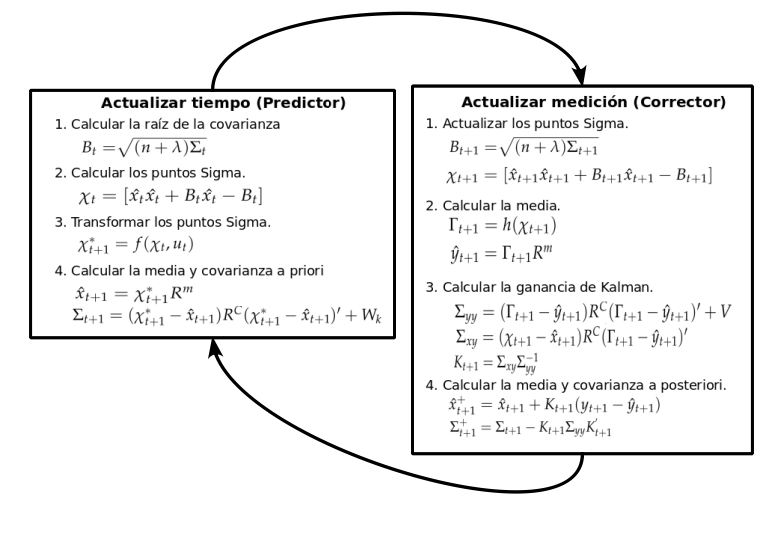
\includegraphics[scale=1.95]{Alg_UKF}
\caption{Iteración UKF \cite{_leyton_2009} \cite{luigi_d&39;alfonso_mobile_2015} .} \label{Iteracion_UKF}
\end{figure}
La idea de este algoritmo es muy parecida a la presentada para el \ac{EKF} con la única diferencia de cómo se propaga la media y la covarianza a través del sistema.
La figura \ref{EKF_UKF_UT} ilustra con un ejemplo sencillo las diferentes formas de propagación de la media y la covarianza para un sistema de dos dimensiones.
En el lado izquierdo se observan la media y la covarianza verdaderas usando el muestreo de Monte Carlo.
En el centro de la figura se muestra el resultado si usaramos la linealización del \ac{EKF}.
Por último, podemos ver el resultado de la transformada \textit{unscented} y como vemos únicamente nos hacen falta 5 puntos para tener una propagación con una media y covarianza representativa.
Si tenemos en cuenta las ideas anteriores podemos ver las similitudes en los algortimos \ref{alg:algoritmoEKF} y \ref{alg:algoritmoUKF} \cite{zhou_ukf_2007}.
\begin{algorithm}
\begin{algorithmic} 
\STATE{$B_{t} = \sqrt[]{(n+\lambda)\Sigma_{t}} $}
\STATE{$\chi_{t} = [\hat{x_{t}}\hat{x_{t}} + B_{t}\hat{x_{t}}-B_{t}]$}
\STATE{$\chi_{t+1}^{*}=f(\chi_{t},u_{t})$}
\STATE{$\hat{x}_{t+1}= \chi_{t+1}^{*}R^{m}$}
\STATE {$\Sigma_{t+1} = (\chi_{t+1}^{*}-\hat{x}_{t+1})R^{C}(\chi_{t+1}^{*}-\hat{x}_{t+1})'+ W_{k} $}
\STATE{$B_{t+1}= \sqrt[]{(n+\lambda)\Sigma_{t+1}}$}
\STATE{$\chi_{t+1} = [\hat{x}_{t+1}\hat{x}_{t+1}+ B_{t+1}\hat{x}_{t+1}-B_{t+1}]$}
\STATE{$\Gamma_{t+1}=h(\chi_{t+1})$}
\STATE{$\hat{y}_{t+1}=\Gamma_{t+1}R^{m}$}
\STATE{$\Sigma_{yy}=(\Gamma_{t+1}-\hat{y}_{t+1})R^{C}(\Gamma_{t+1}-\hat{y}_{t+1})' + V$}
\STATE{$\Sigma_{xy}=(\chi_{t+1}-\hat{x}_{t+1})R^{C}(\Gamma_{t+1}-\hat{y}_{t+1})'$}
\STATE{$K_{t+1}=\Sigma_{xy}\Sigma_{yy}^{-1}$}
\STATE{$\hat{x}_{t+1}^{+}=\hat{x}_{t+1}+K_{t+1}(y_{t+1}-\hat{y}_{t+1})$}
\STATE{$\Sigma_{t+1}^{+} = \Sigma_{t+1}- K_{t+1}\Sigma_{yy}K_{t+1}^{'} $}
\RETURN $\hat{x}_{t+1}^{+},\Sigma_{t+1}^{+}$
\end{algorithmic}
\caption{Algoritmo UKF \cite{_leyton_2009} \cite{luigi_d&39;alfonso_mobile_2015}}\label{alg:algoritmoUKF}
\end{algorithm}

\section{Filtro de Kalman de Cubatura (CKF)}
Cuando afrontamos la estimación de estados en sistemas no lineales, tenemos que dejar de lado la idea de buscar una solución óptima o analítica y debemos conformarnos con una solución subóptima dada por los filtros Bayesianos \cite{_cubature-based_2010} \cite{ienkaran_cubature_2009} \cite{zhang_cubature_2013}.
En términos computacionales una solución subóptima para la densidad de probabilidad a posteriori puede ser obtenida usando una de las siguientes aproximaciones:
\begin{itemize}
\item \textbf{Aproximación local}: En este tipo de aproximación derivamos los filtros no lineales para que la distribución de probabilidad a posteriori tome la forma de la distribución a priori.
Por ejemplo, podemos asumir que se sigue una distribución Gaussiana como hemos hecho en los anteriores filtros (\ac{EKF} y \ac{UKF}).
Este tipo de aproximaciones generan filtros más simples y de una ejecución más rápida.
\item \textbf{Aproximación global}: Aquí no realizamos ningún tipo de suposición específica acerca de la densidad de probabilidad a posteriori. 
Por ejemplo, los filtros de partículas usando integraciones de Monte Carlo con el \textit{sampling importance resampling (SIR)} entra dentro de esta aproximación.
% * <amorellg@ull.edu.es> 2016-06-01T18:28:47.025Z:
%
% > muestro de importancia
%
% esto no lo dejes así literal, ponlo en castellano (en cursiva por ejemplo) y mejor referirse por el original inglés, sampling importance resampling (SIR), me suena raro verlo así traducido vaya :P
%
% ^ <alu0100765755@ull.edu.es> 2016-06-02T11:08:38.922Z.
Normalmente lo métodos globales requieren una gran cantidad de recursos computacionales.
\end{itemize}
Desafortunadamente, los filtros para sistemas no lineales que hemos visto sufren el problema de lo que se conoce como \textit{maldición de la dimensionalidad} además de la \textit{divergencia} \cite{ienkaran_cubature_2009}.
Este efecto puede causar que el filtro vea degradado su rendimiento computacional cuando trabajamos con modelos con una alta dimensión de estados, normalmente con vectores con dimensión superior a 20 estados.
% * <amorellg@ull.edu.es> 2016-06-01T18:31:00.806Z:
%
% > entre en detrimento
%
% mejor "vea degradado su rendimiento computacional"
%
% ^ <alu0100765755@ull.edu.es> 2016-06-02T11:09:51.042Z.
La divergencia puede ocurrir por muchas razones, como podrían ser la imprecisión, un modelo incompleto de nuestro sistema físico o incluso la pérdida de información al capturar la verdadera distribución de probabilidad a posteriori.
Por ejemplo, el \ac{EKF}, que es uno de los filtros más utilizados para sistemas no lineales desde hace décadas trabaja bien en algunas aplicaciones de filtrado que no presenten grandes no linealidades, en caso contrario el sistema presentaría divergencias y el filtro no funcionaría correctamente.

Con la motivación de solucionar el problema anterior surgió lo que se conoce como Filtro de Kalman de Cubatura (CKF).
Como sabemos los filtros Bayesianos son muy fáciles de manejar cuando se asume que todas las densidades de probabilidad son Gaussianas.
De ser así el problema se reduce a calcular integrales multidimensionales cuyos integrandos son de la forma $función no lineal x Gaussiana$.
El \ac{CKF} aprovecha lo que se conoce como las \textit{reglas de cubatura} que sirven para realizar integrales multidimensionales con alta eficiencia de computo.
Con las reglas de cubatura a nuestra disposición podemos describir el funcionamiento del filtro como el filtrado no lineal a través de la teoría estimación lineal, gracias a esta regla de integración el filtro posee su nombre.
El \ac{CKF} se presenta como un filtro numéricamente muy preciso y además fácilmente extensible a problemas de estimación de gran número de dimensiones.

En cuanto a la base matemática el \ac{CKF} presenta muchas similitudes con el \ac{UKF} aunque su ámbito de aplicación es ligeramente distinto.
Ambos métodos usan puntos seleccionados de forma determinista para caracterizar las distribuciones de probabilidad aunque como podremos imaginar estos se hallan de distinta manera para cada filtro.
Recordemos que para el \ac{UKF} seleccionábamos $(2n+1)$ puntos de muestreo con pesos $[\chi_{i},\omega_{i}]_{i=0}^{2n}$ para caracterizar nuestra distribución de probabilidad, siendo $n$ la dimensión del vector de estados.
Para el \ac{CKF} utilizaremos $2n$ puntos para caracterizar nuestra distribución de probabilidad.


\subsection{Transformación esférica-radial}
Como hemos dicho en la sección anterior, el filtrado de sistemas no lineales usando la suposición de distribuciones Gaussianas reduce el problema a cómo calcular las integrales cuyos integrandos son de la forma $función no lineal x Gaussiana$.
Específicamente consideraremos la integral de la siguiente forma:
\begin{equation}\label{Ec:CKF_1}
I(f)=\int_{R^{n}}f(x)exp(-x^{T}x)dx 
\end{equation}
Definida en el sistema cartesiano de coordenadas.
Para calcular el valor numérico de dicha integral lo que haremos será transformarla en la forma esférica-radial, y posteriormente se usará una regla esférica-radial de tercer grado.

En la transformación esférica-radial, el paso clave es cambiar el sistema de coordenadas cartesiano (vector $x$) a un sistema con radio $r$ y vector director $y$.
La transformación sería $x=ry$ donde $y^{T}y=1$, por lo tanto $x^{T}x=r^{2}$.
De esta manera la integral \ref{Ec:CKF_1} puede ser reescrita en el sistema de coordenadas esférico-radial como:
\begin{equation}\label{Ec:CKF_2}
I(f)=\int_{0}^{\infty}\int_{U_{n}}f(ry)r^{n-1}exp(-r^{2})d\sigma(y)dr 
\end{equation}
Donde $U_{n}$ es la superficie de la esfera definida por $U_{n}=[y \epsilon R^{n} \mid y^{T}y=1]$ y $\sigma$ es la superficie esférica medida o lo que es lo mismo, el área de $U_{n}$. 
Podemos escribir la integral radial como:
\begin{equation}\label{Ec:CKF_3}
I=\int_{0}^{\infty}S(r)r^{n-1}exp(-r^{2})dr \approx w_{1}f(x_{1})
\end{equation}
donde $S(r)$ es definido por la integral esférica con la función de unidad de peso $w(y)=1$ que puede ser aproximada por $2n$ puntos \cite{zhang_cubature_2013}:
\begin{equation}\label{Ec:CKF_4}
S(r)= \int_{U_{n}}f(ry)d\sigma(y) \approx w\sum_{i=1}^{2n}f[u]_{i}
\end{equation}
Donde $w>0$ es el peso correspondiente para el generador $[u]$, por lo tanto finalmente tendríamos:
\begin{equation}\label{Ec:CKF_5}
I(f)=\int_{R^{n}}f(x)exp(-x^{T}x)dx = \frac{\sqrt[]{\pi^{n}}}{2n}\sum_{i=1}^{2n}f(\sqrt[]{\frac{n}{2}}[1]_{i})
\end{equation}

Estas integrales esféricas y radiales son normalmente calculadas siguiendo lo que se conoce como \textbf{regla esférica de cubatura} y la \textbf{regla Gaussiana de cuadratura} que pueden ser consultadas en \cite{zhang_cubature_2013} \cite{ienkaran_cubature_2009} \cite{_cubature-based_2010}.

\subsection{Algoritmo del CKF}
\begin{algorithm}
\begin{algorithmic} 
\STATE{$P_{k-1\mid k-1} = S_{k-1\mid k-1}S_{k-1\mid k-1}^{T} $}
\STATE{$X_{i,k-1\mid k-1} = S_{k-1\mid k-1}\xi_{i} + \hat{x}_{k-1\mid k-1}$}
\STATE{$X_{i,k\mid k-1}^{*}= f(X_{i,k-1\mid k-1},u_{k-1})$}
\STATE{$\hat{x}_{k\mid k-1}=\frac{1}{m}\sum_{i=1}^{m}X_{i,k\mid k-1}^{*}$}
\STATE{$P_{k\mid k-1} = \frac{1}{m}\sum_{i=1}^{m}X_{i,k\mid k-1}^{*}X_{i,k\mid k-1}^{*T}-\hat{x}_{k\mid k-1}\hat{x}_{k\mid k-1}^{T} + Q_{k-1} $}
\STATE{$P_{k\mid k-1} = S_{k\mid k-1}S_{k\mid k-1}^{T} $}
\STATE{$X_{i,k\mid k-1} = S_{k\mid k-1}\xi_{i} + \hat{x}_{k\mid k-1}$}
\STATE{$Z_{i,k\mid k-1} = h(X_{i,k\mid k-1},u_{k})$}
\STATE{$\hat{z}_{k\mid k-1}=\frac{1}{m}\sum_{i=1}^{m}Z_{i,k\mid k-1}$}
\STATE{$P_{zz,k\mid k-1} = \frac{1}{m}\sum_{i=1}^{m}Z_{i,k\mid k-1}Z_{i,k\mid k-1}^{T}-\hat{z}_{k\mid k-1}\hat{z}_{k\mid k-1}^{T} + R_{k} $}
\STATE{$P_{xz,k\mid k-1} = \sum_{i=1}^{m}w_{i}X_{i,k\mid k-1}Z_{i,k\mid k-1}^{T}-\hat{x}_{k\mid k-1}\hat{z}_{k\mid k-1}^{T}$}
\STATE{$W_{k}=P_{xz,k\mid k-1}P_{zz,k \mid k-1}^{-1}$}
\STATE{$\hat{x}_{k\mid k} = \hat{x}_{k \mid k-1} + W_{k}(z_{k}-\hat{z}_{k\mid k-1})$}
\STATE{$P_{k\mid k} = P_{k\mid k-1} - W_{k}P_{zz,k\mid k-1}W_{k}^{T}$}
\RETURN $\hat{x}_{k\mid k},P_{k\mid k}$
\end{algorithmic}
\caption{Algoritmo CKF \cite{ienkaran_cubature_2009}}\label{alg:algoritmoCKF}
\end{algorithm}

\begin{figure}[ht!]
\centering
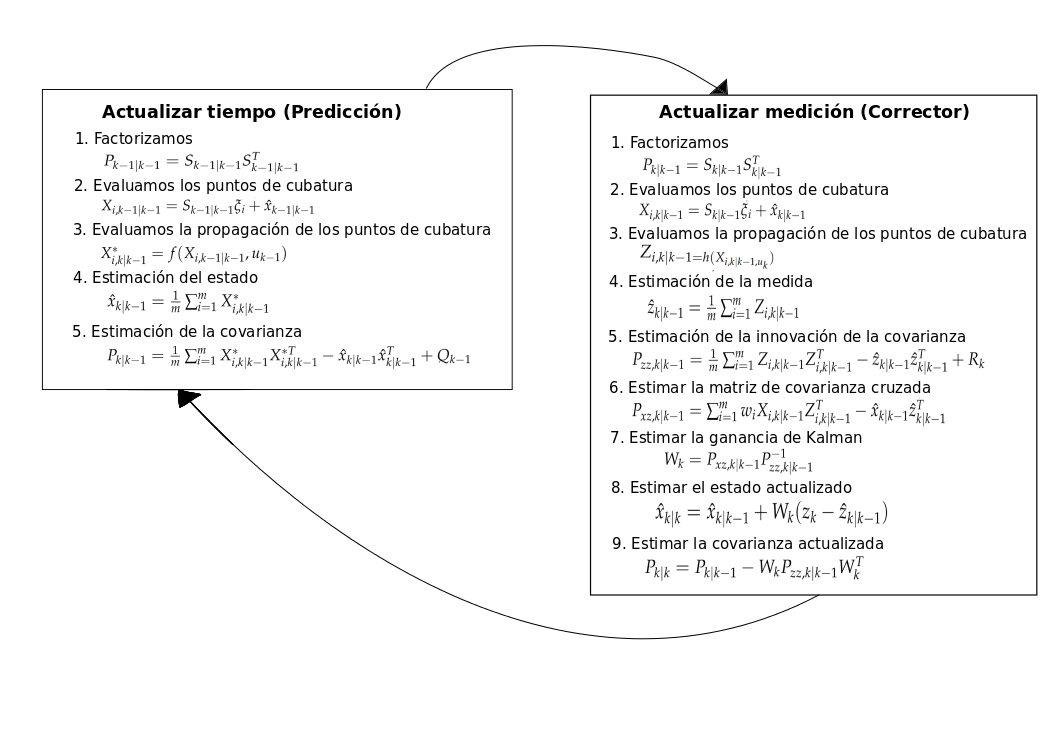
\includegraphics[scale=1.65]{Alg_CKF}
\caption{Iteración CKF \cite{ienkaran_cubature_2009}.} \label{Iteracion_CKF}
\end{figure}
En el algoritmo \ref{alg:algoritmoCKF} y la figura \ref{Iteracion_CKF} podemos ver el funcionamiento básico del \ac{CKF}.
Como en todos los filtros que hemos visto se mantiene la estructura predicción-actualización que permite al filtro funcionar de forma iterativa.
También hay que recordar que para la primera iteración del filtro suponemos que conocemos la densidad de probabilidad del instante anterior, es decir, $p(x_{k+1}\mid D_{k+1}) = \dist{N}(\hat{x}_{k-1\mid k-1},P_{k-1\mid k-1})$.
Una vez vemos el algoritmo \ref{alg:algoritmoCKF} podríamos sacar las siguientes conclusiones acerca del \ac{CKF}:
\begin{itemize}
\item \textbf{La regla de cubatura no utiliza derivadas}. Esta es una propiedad muy útil ya que resalta la necesidad de usar el  \ac{CKF} cuando resulta difícil calcular el Jacobiano o el Hessiano de un sistema.
Esto es un punto a favor frente al \ac{EKF}.
\item \textbf{La regla de cubatura requiere 2n puntos}. Necesitamos 2n puntos de evaluación en cada ciclo del filtro (n es la dimensión del vector de estados).
% * <amorellg@ull.edu.es> 2016-06-01T18:34:09.950Z:
%
% >  2n 
%
% ojo, esto es una exponencial? 2^n ?
%
% ^ <alu0100765755@ull.edu.es> 2016-06-02T11:11:48.860Z:
%
% No, en teoría es una multiplicación . Según el artículo original , en las conclusiones finales que hacen es una de las observaciones.
%
% ^ <amorellg@ull.edu.es> 2016-06-02T17:19:31.156Z:
%
% por si acaso!
%
% ^.
La complejidad computacional escala linealmente conforme aumenta el número de estados.
Estos puntos son usados en los pasos 2 y 3 de ambos ciclos en la figura \ref{Iteracion_CKF}.
En estos pasos se evalúan todos los puntos de cubatura hasta el número 2n.
\end{itemize}
Como vemos el filtro de Cubatura pretende dar un enfoque muy distinto a la estimación de estados en sistemas no lineales, por esta razón se presenta como una posible alternativa cuando la estimación usando el \ac{EKF} o el \ac{UKF} no es posible por tener problemas con la dimensionalidad o las divergencias del sistema.

